\documentclass[11pt]{beamer}
\usepackage{hyperref}
\usepackage[T1]{fontenc}
\UseRawInputEncoding

\usepackage{graphicx}
\usepackage[utf8]{inputenc}
\usepackage{mathtools}
\usepackage{verbatim}
\usepackage{smartdiagram}
\usepackage{unicode-math}
%\setmathfont{}
\usepackage{comment}
\usepackage{xcolor}
% Cannot enable in Xelatex
\usepackage{pgfpages}
% \setbeameroption{hide notes} % Only slides
% \setbeameroption{show only notes} % Only notes
% \setbeameroption{show notes on second screen}
\usepackage{latexsym,amsmath,xcolor,multicol,booktabs,calligra}
\usepackage{graphicx,listings,stackengine}

\usepackage{tikz}
\usepackage{tikz-feynman}
\usepackage[compat=1.0.0]{tikz-feynman}
%\usepackage{float}

%% Enable only in Xelatex
% \usepackage{pstricks}
\usepackage{feynmp-auto} % or feynmp if you prefer
% Feynman diagrams
%\usepackage{feynmp}
%\usepackage{feynmf}
\DeclareGraphicsRule{*}{mps}{*}{} % for being able to read the produced file

\author{Ana Costa Pereira, Joshua Davies}
\title{Parallel Scaling}
%\institute [University of Liverpool]{\href{mailto:Ana.Costa-Pereira@liverpool.ac.uk}{\underline{Ana.Costa-Pereira@liverpool.ac.uk}}}
\date{26/06/2026}
\usepackage{QUT}

% defs
\def\cmd#1{\texttt{\color{red}\footnotesize $\backslash$#1}}
\def\env#1{\texttt{\color{blue}\footnotesize #1}}
\definecolor{deepblue}{rgb}{0,0,0.5}
\definecolor{deepred}{rgb}{0.6,0,0}
\definecolor{deepgreen}{rgb}{0,0.5,0}
\definecolor{halfgray}{gray}{0.55}

\lstset{
    basicstyle=\ttfamily\small,
    keywordstyle=\bfseries\color{deepblue},
    emphstyle=\ttfamily\color{deepred},    % Custom highlighting style
    stringstyle=\color{deepgreen},
    numbers=left,
    numberstyle=\small\color{halfgray},
    rulesepcolor=\color{red!20!green!20!blue!20},
    frame=shadowbox,
}

\setbeamercolor{block body alerted}{bg=alerted text.fg!10}
\setbeamercolor{block title alerted}{bg=alerted text.fg!20}
\setbeamercolor{block body}{bg=structure!10}
\setbeamercolor{block title}{bg=structure!20}
\setbeamercolor{block body example}{bg=green!10}
\setbeamercolor{block title example}{bg=green!20}

\begin{document}
%
%
% Capa
%
%
\begin{frame}
    \titlepage
    \begin{figure}[htpb]
        \begin{center}
           
\includegraphics[width=0.35\linewidth]{logo.png}
           
\includegraphics[width=0.35\linewidth]{logo_livinno.jpg}
        \end{center}
    \end{figure}
\end{frame}


\begin{frame}
    \tableofcontents[sectionstyle=show,subsectionstyle=show/shaded/hide,subsubsectionstyle=show/shaded/hide]
\end{frame}














\begin{frame}{Introduction}
\begin{itemize}
\item Parallel scalings: study of scaling at higher thread number of tform;
\end{itemize}
\textbf{Outline of talk}
\begin{itemize}
\item Overview of sorting process in parallel at the \textcolor{blue}{SortBot} level;
\item Benchmarks performence at different thread count;
\item Changes implemented at the level of \textcolor{blue}{SortBots} and new benchmark results;
\end{itemize}
\end{frame}














\section{SortBot Merging}


\begin{frame}{SortBot Merging}
\small
\begin{itemize}
\item \textcolor{magenta}{Master} $\longrightarrow$ allocations for the workers;
\item \textcolor{orange}{Worker} $\longrightarrow$ independent stream of sorted terms (identical terms live consecutively in memory);
\item  $N$ \textcolor{orange}{workers} $\longrightarrow$ $N-2$ \textcolor{blue}{SortBots} are created; 
\item \textcolor{blue}{SortBots} routine starts; 
\end{itemize}
\begin{figure}
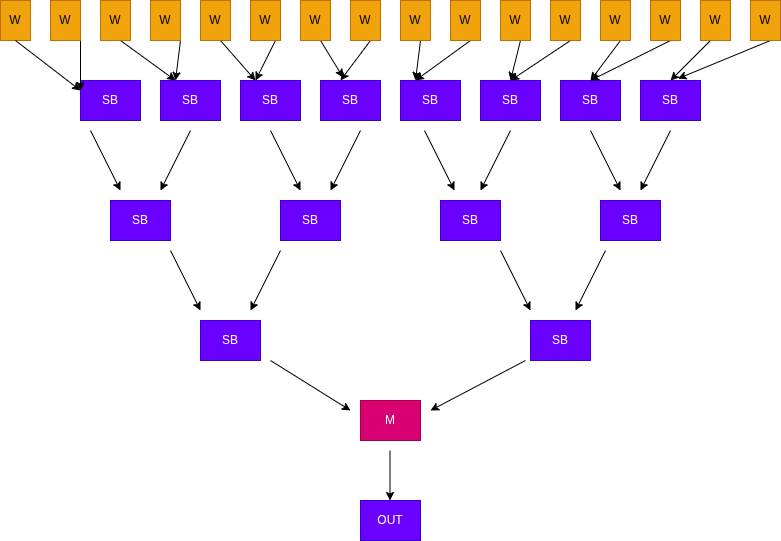
\includegraphics[scale=.20]{images/sb.png}
\end{figure}
\begin{itemize}
    \item \textcolor{magenta}{Master} performs the final merge and writes output.
\end{itemize}
\end{frame}














\section{SortBot Bottlenecks and changes}

\begin{frame}{SortBot: Overlaping of terms}
\begin{itemize}
\item \textcolor{blue}{SortBot} $\longrightarrow$ blocks;
\end{itemize}
\begin{figure}
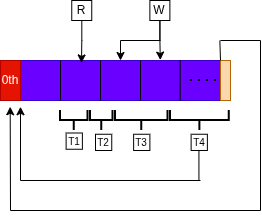
\includegraphics[scale=.50]{images/sb5.png}
\end{figure}
\begin{itemize}
\item Terms are allowed to overlap between blocks;
\item \textcolor{red}{0th block} - the overlap in the end of term is copied to \textcolor{red}{0th block} so that the terms are contiguous.
\end{itemize}
\end{frame}


















\begin{frame}{SortBots Bottlenecks}
\begin{itemize}
\item \textcolor{red}{Bottlenecks}: reading of the input with
\textbf{division of terms} of \textcolor{orange}{workers} to \textcolor{blue}{SortBots}; inverse tree at the end with the
\textbf{writing to the file by the \textcolor{magenta}{Master}};
\end{itemize}
\begin{figure}
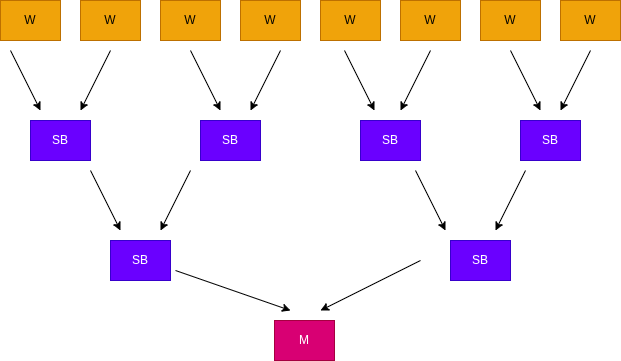
\includegraphics[scale=.3]{images/sb6.png}
\end{figure}
\end{frame}








\begin{frame}
\textcolor{red}{Bottlenecks}
\begin{figure}
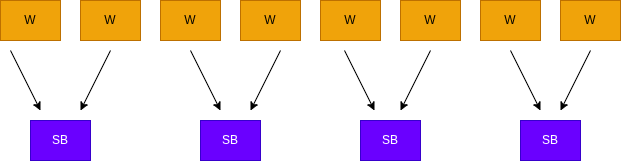
\includegraphics[scale=.30]{images/sb7.png}
\end{figure}
\begin{itemize}
\item Default buffer sized increased $\longrightarrow$ bigger \textcolor{blue}{SortBots}; 
\item overlaping from \textcolor{orange}{worker} fits into \textbf{single block} $\longrightarrow$ SortBotTree mechanism does not paralelize
\item If a \textbf{term} is too big for one block: Worker fills the \textcolor{blue}{SortBots} all the way up to the end of the block, \textbf{overlaping} to the next;
\item Once a block is completely full, it reaches the top and moves on to the next block
\end{itemize}
\end{frame}














\section{Changes in the SortBot Merge}

\begin{frame}{SortBot Block size}
\begin{figure}

\includegraphics[scale=.5]{images/sb8.png}
\end{figure}
\begin{itemize}
\item Decrease the size of the allocations for the \textcolor{blue}{SortBots}: blocks are made smaller;
\item Whole terms must fit into the block: if it does not fit, it goes into the next block;
\item \textcolor{red}{0th block} is obsolete.
\end{itemize}
\end{frame}






\section{SortBot Locking}
\begin{frame}{Locking}
\begin{figure}

\includegraphics[scale=.50]{images/sb3.png}
\end{figure}
\begin{itemize}
\item Writting thread always locks pair of locks - the current thread and the previous thread;
\item Reading threads locks the block where it is reading from;
\end{itemize}
\end{frame}















\begin{frame}{SortBot: Locking}
\begin{figure}
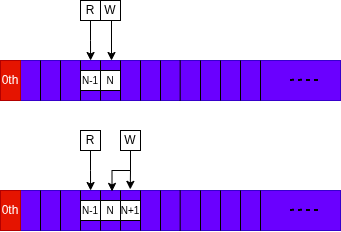
\includegraphics[scale=.50]{images/sb4.png}
\end{figure}
\begin{itemize}
\item Worker (W) detects if there is a Reader (R) waiting for them;
\item W filling the blocks tries to obtain a lock of the block before the current fill block;
\item If W does not obtain the lock, R thread already has the lock - very soon will be done and ready for more terms;
\item The W moves to the next block;
\end{itemize}
\end{frame}






\begin{frame}{SortBot variables}
\begin{itemize}
\item The number of blocks in each SORTBOT has to be at least 4 (due to the locking mechanism) - which corresponds to a minumum of 8 for \textbf{NUMBEROFBLOCKSINSORT};
\item There ia a minimum number of terms that have to fit the block: \textbf{MINNUMBEROFTERMS};
\item Make sure a minimum number of terms is written: never make empty block - \textbf{MINWRITENUMBEROFTERMS};
\end{itemize}
\end{frame}








\begin{frame}
\begin{itemize}
\item \textbf{NUMBEROFBLOCKSINSORT} = 8
\item \textbf{MINNUMBEROFTERMS} = 1
\item \textbf{MINWRITENUMBEROFTERMS} = 1
\end{itemize}
\begin{figure}

\includegraphics[scale=.5]{images/sb9.png}
\end{figure}
\end{frame}










\begin{frame}
Some results after the changes
\begin{itemize}
\item No decrease in performance for any tests;
\item Performance improvement for benchmarks where term merging is expensive (PolyRatFun, PolyRatFunExpand)
\item Forcer, mbox1l
\end{itemize}
\end{frame}











\begin{frame}{SortBots Bottlenecks}
\textcolor{red}{Bottlenecks}
\begin{figure}
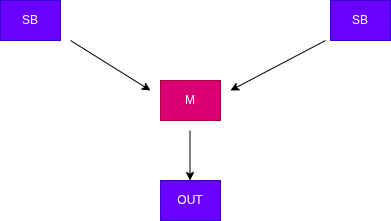
\includegraphics[scale=.30]{images/sb1.png}
\end{figure}
\begin{itemize}
\item End of the tree: \textcolor{magenta}{Master} performs last sorting as well as writting of terms into the output;
\item Performance could be increased by having one last stage of sorting of tha last 2 \textcolor{blue}{SortBots} and \textcolor{magenta}{Master} only writting;
\end{itemize}
\end{frame}








\begin{frame}{Adition of new SortBot}
\begin{itemize}
\item Add a new SortBot at the end of the merging tree to do the sort of the streams that comes from last 2 SortBots;
\item Master only does the writting.
\end{itemize}
\begin{figure}
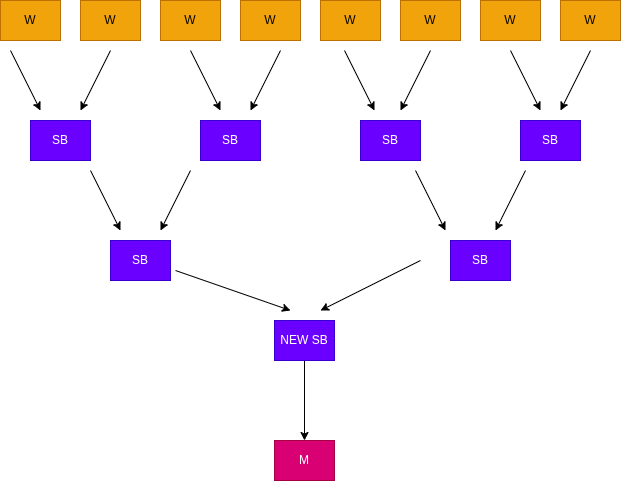
\includegraphics[scale=.3]{images/sb10.png}
\end{figure}
\end{frame}







\end{document}
